A Figura~\ref{fig:comparacao_crescente} apresenta a comparação entre
os sete algoritmos para entradas inicialmente ordenadas de forma
crescente.

\begin{figure}[H]
    \centering
    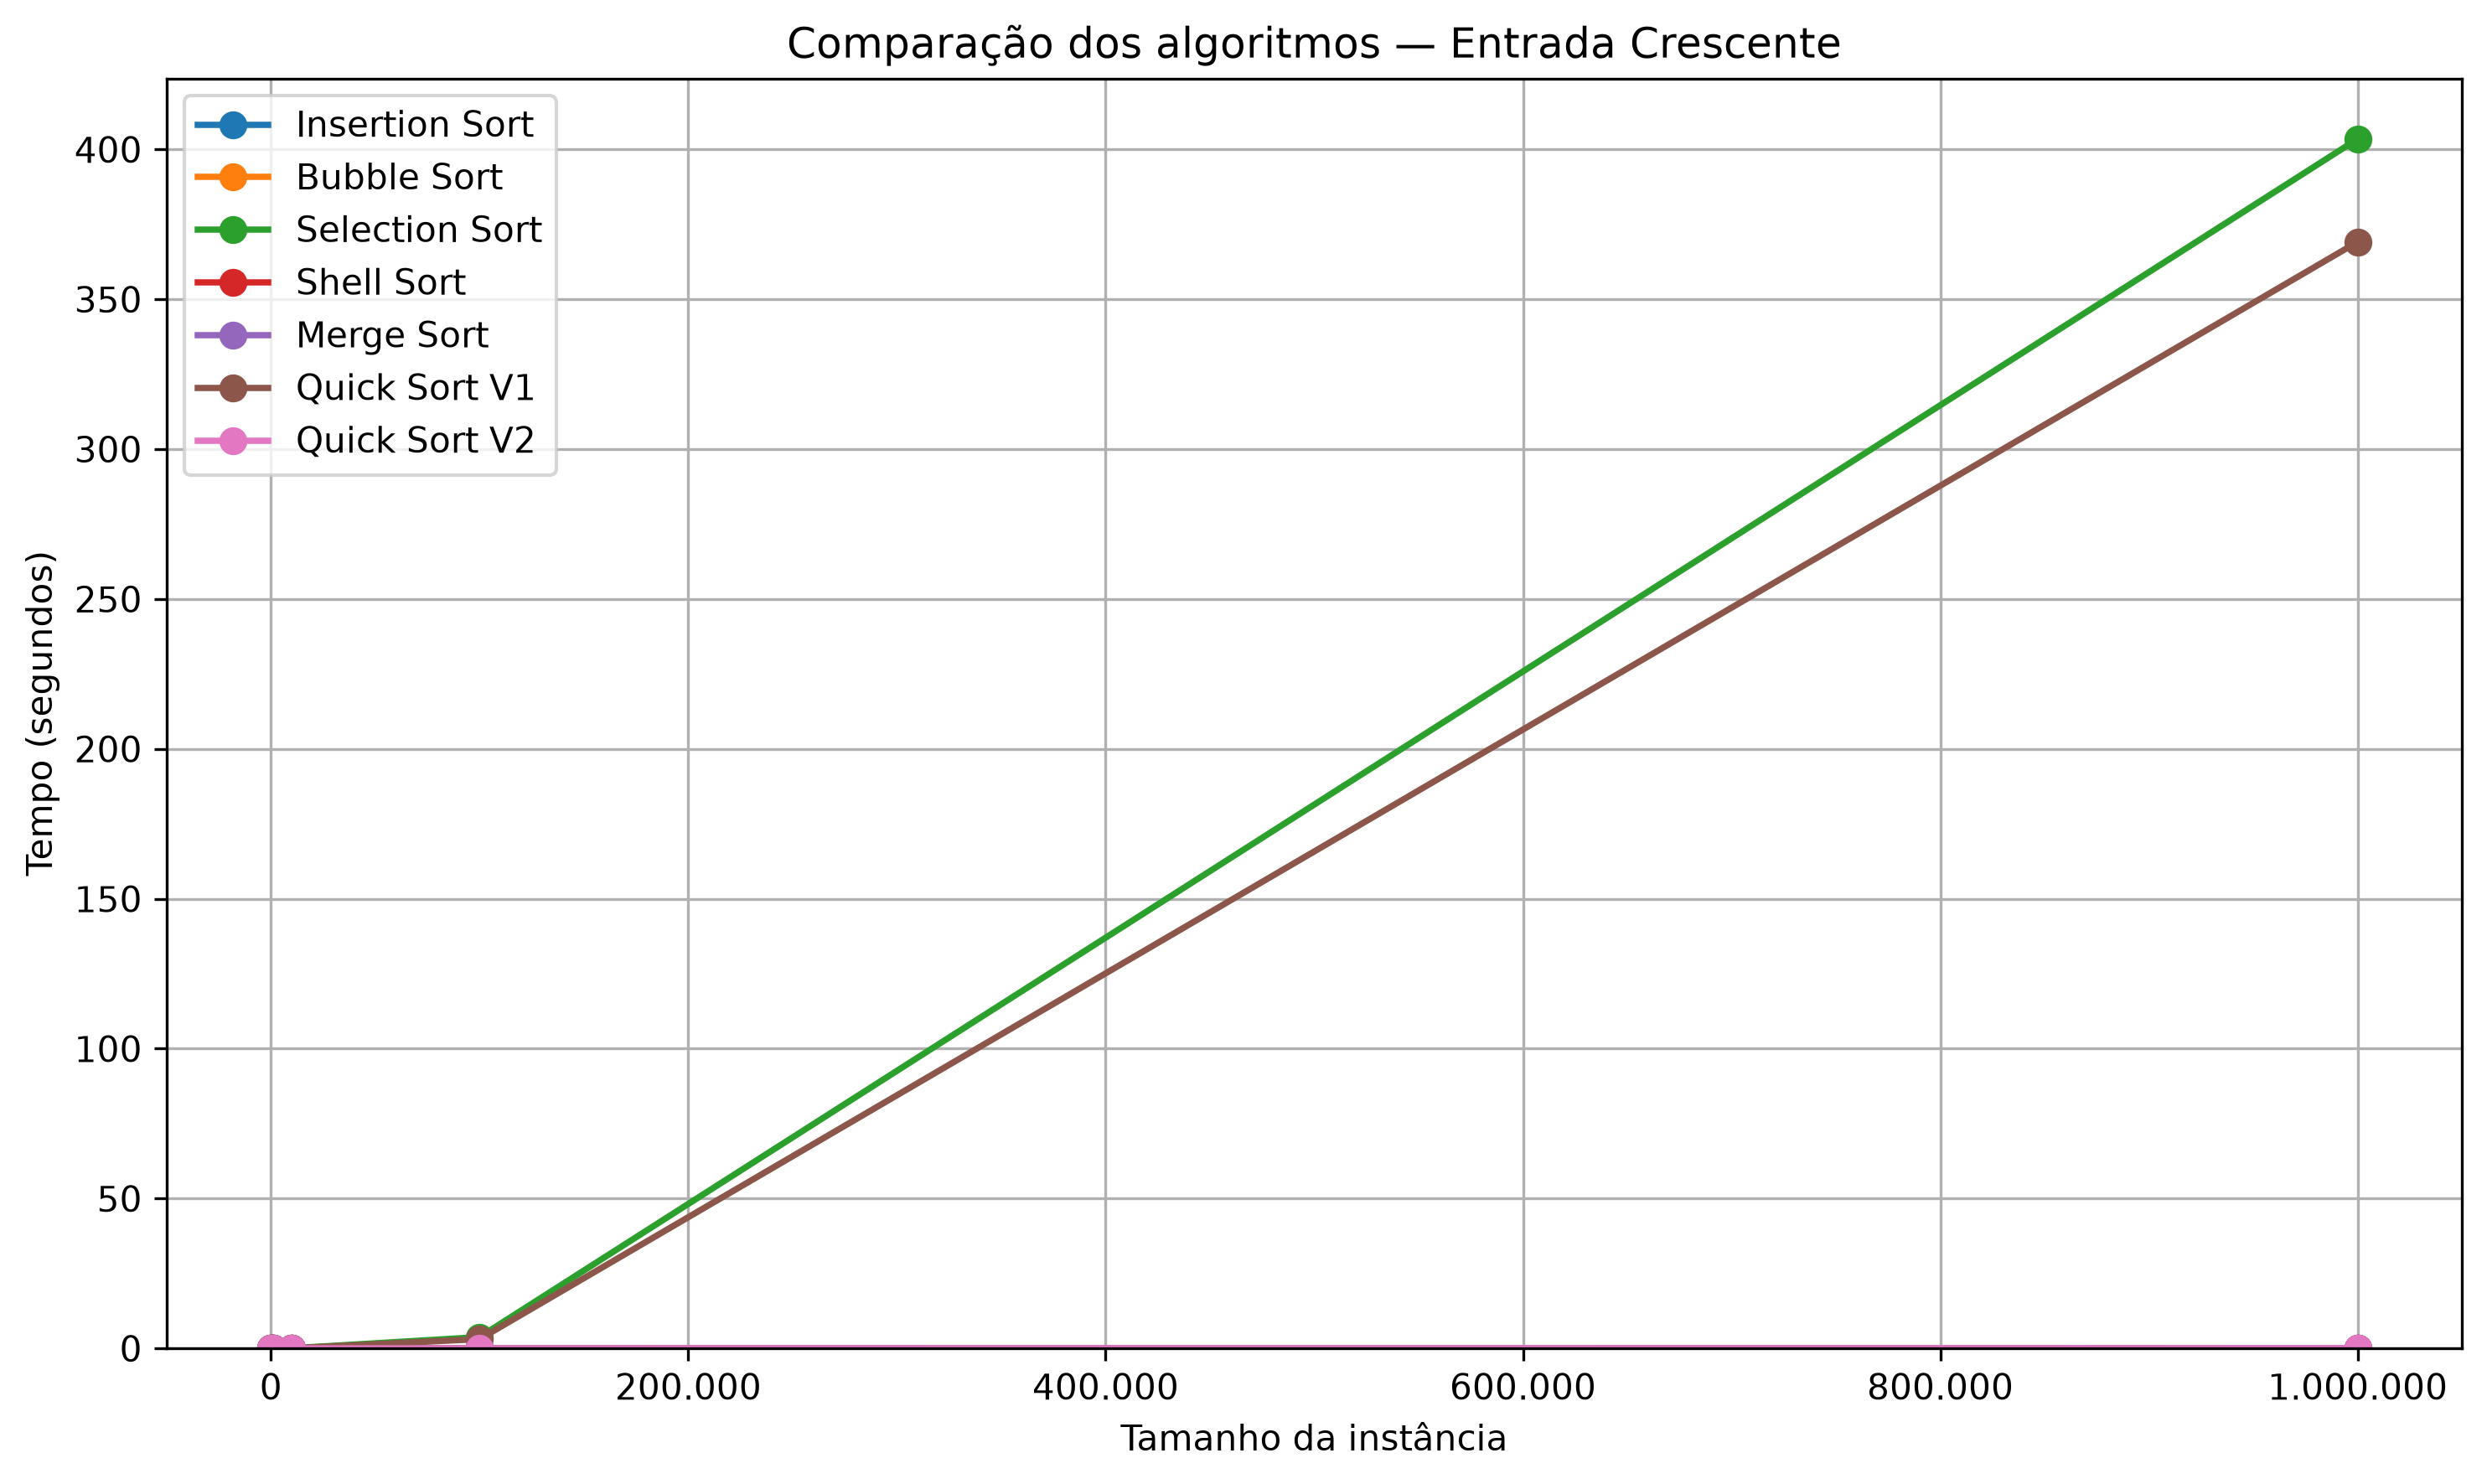
\includegraphics[width=\textwidth,keepaspectratio]{Imagens/Comparacoes/comparacao_crescente.png}
    \caption{Comparação dos algoritmos para entrada crescente.}
    \label{fig:comparacao_crescente}
\end{figure}

Nesse tipo de entrada, apenas dois algoritmos apresentaram tempos
elevados: o \textit{Selection Sort}, com cerca de 400 segundos para
1.000.000 de elementos, e o \textit{Quick Sort} versão 1, com cerca de
370 segundos. O \textit{Selection Sort} mantém uma quantidade quadrática
de comparações mesmo com o vetor já ordenado, pois sempre percorre a
parte não ordenada para localizar o menor elemento. Já o \textit{Quick
Sort} versão 1 utiliza o primeiro elemento como pivô, que em um vetor
crescente é sempre o menor valor da partição. Dessa forma, cada
particionamento separa apenas um elemento, e o algoritmo se comporta de
acordo com o pior caso, $\Theta(n^2)$.

O \textit{Insertion Sort} e o \textit{Bubble Sort} apresentaram tempos
praticamente nulos na escala do gráfico, pois, em vetores já ordenados,
o primeiro não precisa deslocar elementos e o segundo é interrompido
antecipadamente quando não ocorrem trocas, ambos com custo linear. O
\textit{Shell Sort} e o \textit{Merge Sort} também apresentaram tempos
muito baixos, compatíveis com a complexidade próxima de $\Theta(n\log n)$.

A versão 2 do \textit{Quick Sort} não sofreu a degradação observada na
versão 1. Como a média aritmética de valores distribuídos
uniformemente fica próxima do centro da partição, as partições
permaneceram equilibradas mesmo com o vetor ordenado, e o tempo de
execução foi comparável ao do \textit{Merge Sort}. Esse resultado mostra
que a escolha do pivô é decisiva para o desempenho do algoritmo.
